% Sources: comparison-final/*/comparison-table.json and matching repeat/settings.json;
% representation/*/summary.csv; exact-code-groups/group-summary.csv and selection-provenance.json.
The clearest bitplane result is Quora with 32-bit Qwen codes and one returned result. After giving all methods clusters trained on the binary document vectors, B takes 0.081 ms at 99.2\% recall, compared with A's 0.195 ms and C's 0.169 ms at 99.0\%. These are repeated times for the exact settings selected in the main runs, using all 1,000 queries.

\begin{center}\small
\begin{tabularx}{\linewidth}{@{}lrrYrrr@{}}\toprule
Method & Clusters & Probes & Local setting & Recall & ms & Rows scored\\\midrule
A & 4096 & 180 & Scan opened rows & 99.00\% & 0.195 & 24,181.1\\
B & 16 & 9 & Leaf 128; budget 8192; deeper ties & 99.20\% & 0.081 & 817.8\\
C & 1024 & 78 & Start 4; target 0; exact stop & 99.00\% & 0.169 & 26,153.5\\\bottomrule
\end{tabularx}
\end{center}
Rows scored is the mean per query; time is the median over the three repeated processes' 3,000 query observations. B opens clusters containing about 295,031 rows but scores only 818 of them, while visiting about 53,693 split-mask words. Its three process medians range from 0.08025 to 0.08167 ms, below A's 0.19223--0.19708 ms and C's 0.16781--0.16994 ms. B's finite budget still makes this an approximate setting: 99.2\% is the observed recall, not an exactness guarantee. C's bound proves the answer within its opened clusters; routing can still exclude a global neighbor.

\begin{figure}[htbp]
\centering
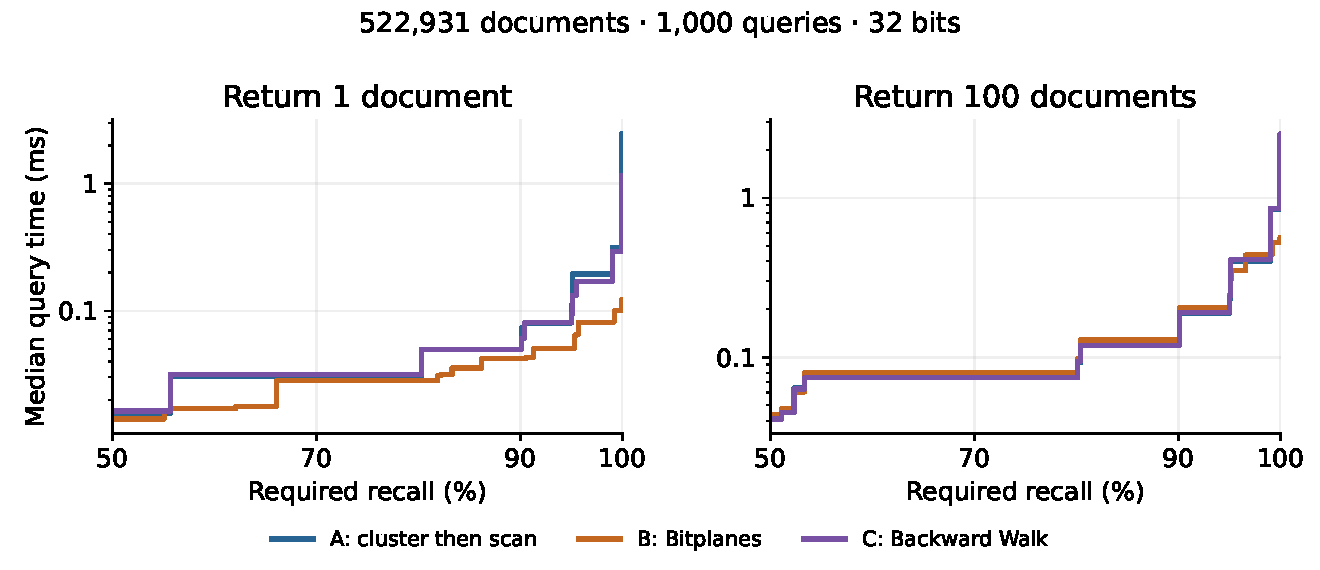
\includegraphics[width=\linewidth]{figures/qwen32-comparison.pdf}
\caption{Qwen32 recall and query time, starting from cached vectors. The vertical axes use a log scale. The curves choose the fastest completed settings meeting each recall; the tables use their repeated timings.}
\label{fig:qwen32-comparison}
\end{figure}

If we ask for 100 results, the conclusion changes. The table below uses the same 99\% recall requirement for every method and reports the repeated median of its selected setting.

\begin{center}\small
\begin{tabular}{@{}llrrr@{}}\toprule
Collection/model & Bits & A (ms) & B (ms) & C (ms)\\\midrule
MS MARCO/Nomic & 64 & 1.915 & 2.071 & \textbf{1.875}\\
MS MARCO/Nomic & 256 & \textbf{13.453} & 13.866 & 14.645\\
MS MARCO/Nomic & 768 & \textbf{45.088} & 45.217 & 45.196\\
Quora/Qwen & 32 & \textbf{0.400} & 0.439 & 0.404\\
Quora/Qwen & 256 & \textbf{3.564} & 3.721 & 4.039\\
Quora/Qwen & 1024 & \textbf{22.863} & 23.098 & 22.930\\\bottomrule
\end{tabular}
\end{center}
Every entry reaches at least 99\% recall again in its repeats. At these selected settings, B does no splitting and C starts at depth zero. Within each row, all three methods use the same 4096-cluster layout, probe count and number of document scores. C has a slightly lower median on Nomic64, but it avoids no scores there. Small timing differences between these scan-like paths do not establish a pruning advantage.

The earlier Qwen32 top-100 lead for B disappears when A also receives the binary-trained layouts. With the stronger routing, A opens 380 clusters and scores about 50,865 rows at 0.400 ms; B and C score the same rows at 0.439 and 0.404 ms. For one result, however, B's pruning advantage remains, and C also beats the best tested A setting, although B is faster overall. This is why I compare each method with A's own selected settings rather than only holding A at one convenient probe count.

\textbf{Code length.}
The 32-bit result answers a different ranking question from the full 1024-value embedding. To measure that difference, I find the best full-float score over the entire corpus, then rescore each width's exact binary top 100 using those full vectors. ``Agrees'' means its score is within $10^{-5}$ of the full-float best; equal-score documents need not have the same ID.

\begin{center}\small
\begin{tabular}{@{}llrr@{}}\toprule
Model/collection & Bits & \shortstack{Binary top 1\\agrees} & \shortstack{Best score reached\\within binary top 100}\\\midrule
Qwen/Quora & 32 & 14.0\% & 73.0\%\\
Qwen/Quora & 256 & 75.8\% & 100.0\%\\
Qwen/Quora & 1024 & 88.6\% & 100.0\%\\
Nomic/MS MARCO & 64 & 17.6\% & 65.6\%\\
Nomic/MS MARCO & 256 & 48.0\% & 97.2\%\\
Nomic/MS MARCO & 768 & 70.2\% & 99.9\%\\\bottomrule
\end{tabular}
\end{center}
For Qwen32, even the exact binary top-1 answer reaches the full-float best score on only 14\% of queries. Keeping the binary top 100 raises that to 73\%, compared with 100\% at 256 bits. So a faster, high-recall search over 32-bit codes does not by itself preserve full-embedding results. These are score-agreement diagnostics, not human relevance scores or measured end-to-end quality for B or C. An approximate search may also miss some of those exact binary candidates.

\textbf{Exact code matches.}
A separate global experiment removes routing entirely and requires the exact best binary result. I select one setting per method on all 1,000 Qwen32 queries, then split those same repeated observations by whether the query's full 32-bit sign pattern exists in the corpus. There are 82 such queries and 918 without a matching code. The settings are not retuned for either group: B uses leaf 2048 with no node limit, and C starts at 32 with target zero and the exact-stop bound.

\begin{center}\small
\begin{tabular}{@{}lrrrr@{}}\toprule
Query group & Queries & A ($\mu$s) & B ($\mu$s) & C ($\mu$s)\\\midrule
All queries & 1000 & 2481.667 & 124.084 & 1163.521\\
Complete code present & 82 & 2481.250 & 128.521 & 4.875\\
Complete code absent & 918 & 2481.708 & 123.750 & 1170.730\\\bottomrule
\end{tabular}
\end{center}
All three methods return the exact binary result in every group. On the 82 matching-code queries, C scores only 1.68 rows on average and stops after its first pair of boundary searches. This is a real case where direct prefix lookup helps. A matching binary code does not imply identical text. But on the remaining 918 queries, it scores about 303,177 rows on average while widening the prefix. B therefore remains faster over the full 1,000-query batch. The 4.875 $\mu$s result belongs to that 8.2\% subgroup under the same global settings; it is not C's overall time or a comparison with separately tuned subgroup indexes.
